\chapter{Fundamentação teórica}

\section{Desenvolvimento de software} % (fold)
\label{sec:desenvolvimento_de_software}

% section desenvolvimento_de_software (end)

\subsection{Métodos tradicionais} % (fold)
\label{sub:metodos_tradicionais}

A base para diversos métodos de desenvolvimento que vêm sendo utilizado há décadas na indústria do software $-$ por isso métodos tradicionais $-$ é o modelo em cascata. Ele sugere uma abordagem sistemática e sequencial para o desenvolvimento de software que começa com a especificação dos requisitos pelo cliente e progride ao longo do planejamento, modelagem, construção, e implantação, culminando na manutenção progressiva do software acabado \cite{Pressman}.

\citeonline{XPTeles} e \citeonline{BDDRodrigo} fazem um apanhado sobre a relação entre o modelo cascata com os processos de produção industriais tayloristas. Estes processos tem como premissas o determinismo e a especialização. Dessa forma, isso leva ao desenvolvimento em cascata a especializar o desenvolvimento, ou seja, separar papéis na equipe de desenvolvimento onde cada um tem uma única responsabilidade. Além disso, existe uma busca pelo determinismo, que ganha força ao ser amparado pelo famosa curva de custos de correção do software por tempo transcorrido desde o início do processo \cite{Boehm}, mostrada na Figura \ref{img:custo-cascata}.

\begin{figure}[h]
  \center
  \caption{O custo das modificações no modelo tradicional - Fonte: \cite{XPKent}}
  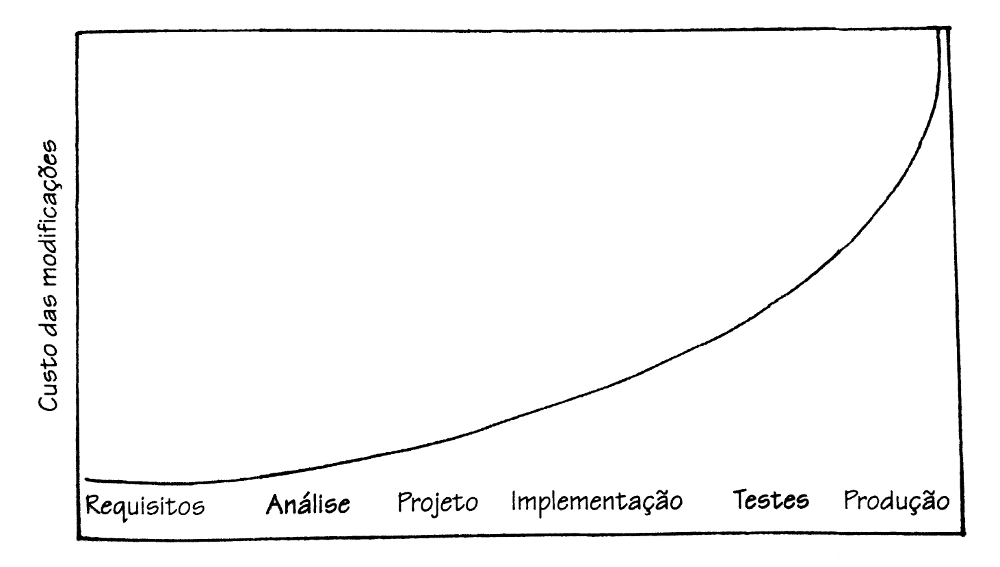
\includegraphics[scale=0.35]{images/custo-cascata}
  \label{img:custo-cascata}
\end{figure}

Esta busca pelo determinismo fez com que se pensasse, de forma completamente equivocada, que ao tentar com bastante afinco, consegue-se antecipar todo o conjunto de requisitos e reduzir os custos eliminando as mudanças \cite{TheBusinessOfInnovation}.

Ainda se baseando no processo de produção industrial, desta vez no gerenciamento fordista, outra premissa extremamente equivocada englobada pelo modelo cascada é a de que desenvolvimento de software é um trabalho executado por trabalhadores manuais e não um trabalhadores do conhecimento \cite[38]{XPTeles}.

Embora o desenvolvimento em cascata seja reconhecidamente ineficaz, ainda é o processo mais utilizado para o desenvolvimento de sistemas \cite{XPTeles}.

% subsection metodos_tradicionais (end)


\subsection{Agilismo} % (fold)
\label{sub:agilismo}

Atividades como escrever um livro, pintar um quadro ou esculpir uma escultura são atividades quase essencialmente intelectuais. Estas atividades possuem três características fundamentais \cite{XPTeles}:

\begin{itemize}
  \item \textbf{Necessidade de revisões}: Ao escrever um livro, o autor revisa e corrige o texto diversas vezes até que a obra adquira sua forma final, De maneira semelhante, um escultor faz diversos retoques até que sua escultura esteja finalizada.
  \item \textbf{Ausência de linearidade}: Dificilmente um autor começa o livro no primeiro capítulo e segue escrevendo até o último, um capítulo de cada vez, na mesma sequencia em que aparecem no índice. Igualmente, é improvável que um escultor ao esculpir uma obra siga um caminho linear.
  \item \textbf{Ausência de determinismo}: Não é possível dizer os passos exatos que o autor seguirá para produzir uma obra, muito menos a ordem em que estes passos serão dados. Cada autor segue um caminho distinto.
\end{itemize}

Segundo \citeonline{XPTeles}, estas características se originam no fato de o autor aprender enquanto produz e esse aprendizado vem do \textit{feedback} que a obra fornece para seu criador, como se houvesse um diálogo permanente entre eles. Na medida em que ele a avalia, a obra mostra ao autor os pontos que precisam ser aprimorados ou necessitam de adições. Em síntese, o trabalho intelectual se caracteriza por aprendizado  permanente que leva a melhorias e torna o produto final mais adequado para o seu público.

O desenvolvimento de software é essencialmente uma atividade intelectual e criativa, exigindo a manipulação de uma gama muito grande de conhecimentos e informações. Além disso, além do autor de um software se preocupar com o conteúdo e estrutura, ele deve ser preocupar também com o comportamento, diferente da escrita de um livro ou da criação de uma escultura, fazendo com o que o desenvolvimento de software seja ainda mais complexo que estas atividades.

Sendo assim, o desenvolvimento de software tem uma semelhança muito maior com a prestação de serviços $-$ e até mesmo com atividades artísticas $-$ do que com manufaturas fordistas. Isto confirma que o desenvolvimento de software seja uma atividade que deve ser realizada por trabalhadores do conhecimento, não por trabalhadores manuais.

Em 2001 um grupo de dezessete especialistas, reconhecidos pela comunidade como grandes nomes do desenvolvimento software, se reuniram para discutir sobre um crescente conjunto de métodos que vinham surgindo e decidiram usar o termo Agilismo para descrever essa nova geração de métodos ágeis \cite{AgileStory}. Na mesma reunião, eles também escreveram o Manifesto Ágil \cite{AgileManifesto}, delineando um conjunto de valores e princípios que, em resumo, trilham um caminho para a eliminação de documentação e processos desnecessários, buscando a simplicidade, com foco na geração de valor e proximidade com o cliente, além de possibilitar respostas rápidas e eficazes às mudanças. O foco, antes fixado no processo, passa a ser nas pessoas e as mudanças, antes fortemente evitadas, são abraçadas.

Pode-se dizer então, que o Desenvolvendo Ágil, ou Agilismo, é um rótulo genérico para os métodos de desenvolvimento de software baseados no Manifesto Ágil \cite{BDDRodrigo}.

É importante citar que o desenvolvimento ágil sofreu grande influência de um conceito conhecido como \textit{Lean Thinking} (``pensamento enxuto"\ em português), uma linha de pensamento em gestão baseada nos princípios de \textit{Lean Manufactoring}\footnote{Os princípios de \textit{Lean Manufactoring} são originários do sistema Toyota de produção, que propôs um modo inteiramente novo de pensar a respeito de fabricação e logística de automóveis.} que se caracteriza por produção em pequenos lotes, eliminação de desperdícios, obsessão com qualidade, equipes multifuncionais praticando aprendizado contínuo, melhoria contínua de processo, sistema puxado de produção e a qualidade sendo responsabilidade dos trabalhadores como um todo \cite{BDDRodrigo}.

Uma das premissas do agilismo é que o custos de alterações é praticamente linear ao longo do tempo, independente do ponto em que esteja, fazendo com que a curva de custo de alterações seja semelhante à apresentada na Figura \ref{img:custo-agile}.

\begin{figure}[h]
  \center
  \caption{O custo das modificações no modelo ágil - Fonte: \cite{XPKent}}
  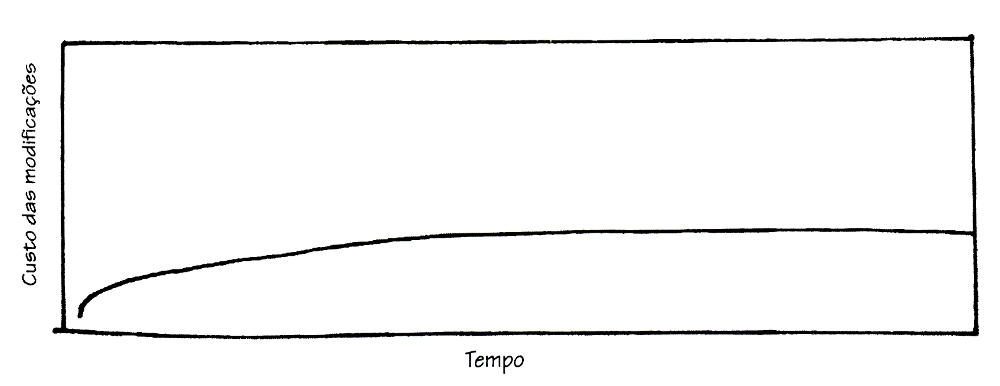
\includegraphics[scale=0.45]{images/custo-agile}
  \label{img:custo-agile}
\end{figure}

Isto é conseguido porque, diferentemente dos métodos tradicionais, os métodos ágeis não fazem um planejamento inicial muito abrangente. Ao invés disso, o desenvolvimento é dividido em iterações curtas (de uma a quatro semanas), onde ao início de cada uma delas é feito um novo planejamento, corrigindo o curso do projeto com base no \textit{feedback} obtido nas iterações anteriores. Para isso, a proximidade e interação do cliente com o projeto deve ser constante. Desta forma, o desenvolvimento é baseado em \textit{feedback} concreto e não em especulações sobre o futuro, o que é comum nos métodos tradicionais \cite{BDDRodrigo}.

\citeonline{MestradoTeles} cita um estudo em que os resultados mostram que 45\% das funcionalidades implementadas nunca são utilizadas, 19\% são raramente utilizadas, 16\% às vezes, 13\% frequentemente e apenas 7\% das funcionalidades são utilizadas sempre. Ou seja, 45\% do trabalho é totalmente inútil, enquanto apenas 20\% é a parte que gera mais retorno para o cliente. Isto é um outro efeito do grande planejamento inicial feito nos métodos tradicionais. Como o cliente tem apenas uma oportunidade para dizer o que ele precisa, sem nem mesmo saber direito o que é. Isso não ocorre nos métodos ágeis, pois a cada iteração o cliente aprende ao ver o que foi produzido nas iterações anteriores $-$ software realmente funcionado $-$ e pode dizer com muito mais certeza o que ainda é necessário ser desenvolvido.

Ao utilizar métodos ágeis, mais especificamente no \textit{eXtreme Programming} (XP), todas as funcionalidades dos sistema são levantadas através de histórias, que são escritas pelo próprio cliente em pequenos cartões. A equipe de desenvolvimento utiliza os cartões para saber quais funcionalidades são desejadas pelo cliente. Contudo, os cartões podem acabar representando histórias que consomem muito esforço para serem implementadas. Nesse caso, a equipe divide os cartões em tarefas, que são registradas em novos cartões para serem distribuídas facilmente entre os desenvolvedores.

No início do projeto o cliente e a equipe de desenvolvimento dividem o projeto em \textit{releases}, que são entregas de software que implementem um conjunto de funcionalidades que possui um valor bem definido para o cliente. Essas entregas são feitas de forma incremental, e em um curto espaço de tempo (geralmente dois meses), para que o cliente possa começar a utilizar e obter os benefícios que elas oferecem, além de dar o \textit{feedback} necessário para que sejam feitas melhorias. Depois de definida a primeira \textit{release}, o cliente escreve as histórias que serão implementas nesta. As histórias das \textit{releases} posteriores podem ser deixadas para o futuro, pois durante o desenvolvimento de cada \textit{release} o cliente irá utilizar o software diversas vezes, o que irá influenciar as histórias das próximas \textit{release}. Durante a \textit{release} o cliente pode alterar as histórias se considerar necessário, podendo assim incorporar o aprendizado adquirido com o uso do sistema.

Uma \textit{release}, mesmo que seja pequena, representa um tempo ainda grande. Assim, ela é dividida em um conjunto de iterações, que são basicamente um pequeno espaço de tempo (geralmente duas semanas) dedicado para a implementação de um conjunto de histórias. A diferença entre uma \textit{release} e uma iteração é que na iteração o cliente não pode alterar as histórias definidas, pois a mudanças muito frequentes ao longo do trabalho da equipe de desenvolvimento prejudicam o ritmo de programação, pois confundem os desenvolvedores. No início de cara iteração é feita uma reunião para o planejamento da mesma, de modo que cliente e equipe de desenvolvimento definam as histórias que serão implementadas na iteração. Ao final de cada iteração e cada \textit{release}, o cliente ter novas histórias implementadas, ou seja, software funcionando. Dessa forma, ele poderá utilizar o sistema com as novas funcionalidades, tornando o \textit{feedback} é ainda mais efetivo.

Mas para que isso seja possível, os métodos ágeis contam com um conjunto de técnicas para dar suporte à seu caráter iterativo e incremental, sendo algumas destas técnicas serão abordadas mais adiante neste trabalho.

% subsection agilismo (end)

% section desenvolvimento_de_software (end)

\section{Teste de software}
\label{sec:teste_de_software}


A maneira como o teste de software é aplicado varia de acordo com a metodologia utilizada no desenvolvimento. Tradicionalmente o teste de software é feito somente após o desenvolvimento ter sido concluído. Já no métodos ágeis um caminho oposto é seguido, sendo utilizadas técnicas como \textit{Test-Driven Development} (abordada na Seção \ref{sec:tdd}) e  \textit{Behaviour-Driven Development} (abordada na Seção \ref{sec:bdd}).

Contudo, apesar de seguirem caminhos opostos, no desenvolvimento ágil é possível e desejável utilizar técnicas de teste de software oriundas e utilizadas no modelo tradicional, como classes de equivalência, análise do valor limite e análise da complexidade ciclomática.

Na literatura existem variadas nomenclaturas e definições para os diferentes tipos de teste. Dessa forma, os próximos tópicos definirão quais serão utilizadas durante o presente trabalho.

\subsection{Testes de unidade}
\label{sub:testes_de_unidade}

Testes de unidade são testes nos quais unidades individuais do sistema são testadas para determinar se estão aptas para uso. Uma unidade é a menor parte testável de uma aplicação. Em programação procedural uma unidade pode ser uma função ou \textit{procedure}. Já em programação orientada a objetos, uma unidade pode ser um método. \citeonline{TesteSoftware} afirmam que neste contexto, espera-se que sejam identificados erros relacionados a algoritmos incorretos ou mal implementados, estruturas de dados incorretas, ou simplesmente erros de programação.

Para exemplificar, no Código \ref{code:unit_test_spec} é apresentado o de teste de unidade para o método \texttt{Category\#name\_as\_css\_class}, cuja implementação é mostrada no Código \ref{code:unit_test}. Como se pode perceber, este método transforma o nome da Categoria em um nome de classe CSS\footnote{\textit{Cascading Style Sheets}. Mais em \url{http://pt.wikipedia.org/wiki/Cascading_Style_Sheets}}, deixando todos seus caracteres em minúsculo e substituindo os caracteres / (barra),  (espaço) e - (traço) por \_ (sublinhado).

\begin{mycode}{rspec}%
{Teste de unidade automatizado para o método \texttt{Category\#name\_as\_css\_class} }{code:unit_test_spec}
# spec/models/category_spec.rb
describe Category do
  it "should return its name as a css class" do
    category = Factory.build :category, :name => "Feature"
    category.name_as_css_class.should == "feature"

    category.name = "New Feature"
    category.name_as_css_class.should == "new_feature"

    category.name = "Other-New Feature"
    category.name_as_css_class.should == "other_new_feature"

    category.name = "Study/Research"
    category.name_as_css_class.should == "study_research"
  end
end
\end{mycode}

\begin{mycode}{rspec}%
{Implementação do método \texttt{Category\#name\_as\_css\_class} }{code:unit_test}
# app/models/category.rb
class Category < ActiveRecord::Base
  def name_as_css_class
    self.name.downcase.gsub(/\/| |-/, "_")
  end
end
\end{mycode}

É interessante observar a diferença entre a utilização e não utilização do TDD, tendo em vista um aviso feito por \citeonline{Pressman}: ``Há algumas situações em que você não terá recursos para fazer teste de unidade abrangente. Selecione módulos críticos e aqueles que têm complexidade ciclomática alta e faça o teste de unidade apenas neles.". Em uma situação onde o TDD é estritamente utilizado, um aviso como esse se torna sem sentido e soa completamente anacrônico. Além disso, ao encontrar algum ponto onde a complexidade ciclomática esteja alta, o aconselhável é que esta seja diminuída através de refatoração, e não apenas testada. Mais sobre TDD na Seção \ref{sec:tdd}.

% subsection testes_de_unidade (end)

\subsection{Testes de integração}
\label{sub:testes_de_integracao}

No contexto do presente trabalho, os testes de integração testam as integrações do código com o mundo exterior. Eles podem ser testes que se comunique através da rede, tenha contato com o sistema de arquivos ou deixe os limites de seu próprio processo \cite{ArtOfAgileDevelopment}.

Para exemplificar, será utilizada uma extensão criada para fazer o \textit{highlighting} de código na descrição das Tarefas e no conteúdo do Comentários no kanban-roots. Para isso, é utilizado um \textit{framework} em Python chamado Pygments\footnote{ Mais em \url{http://pygments.org/}}.

O Pygments deve ser instalado na máquina onde o kanban-roots está sendo executado. No entanto, o kanban-roots foi projetado rodar em um servidor próprio ou em um VPS\footnote{ \textit{Virtual Private Server}. É um servidor em ambiente compartilhado que possui acesso \textit{root} e processos independentes para cada conta VPS criada.}, mas também no Heroku\footnote{ É um PaaS (\textit{platafom as a service}) que tem uma cota de utilização gratuita. No Heroku não é possível instalar dependências no sistema. Mais em \url{http://heroku.com}}. Sendo assim, foi utilizado um serviço gratuito e não oficial criado por Trevor Turk e hospedado no Google App Engine que permite a utilização da API do Pygments através de um POST para o serviço. Dessa forma, deve-se testar a integração com o serviço e também a integração com o Pygments instalado localmente.

\begin{mycode}{rspec}%
{Teste de integração automatizado para o \textit{highlighting} de código}{code:integration_spec}
# spec/lib/albino_render_spec.rb
describe HTMLwithAlbino do
  before(:all) do
    @render = HTMLwithAlbino.new
    @code_text = 'puts "hello!"'
    @highlighted_code =
      "<div class=\"highlight\"><pre>" +
        "<span class=\"nb\">puts</span> <span class=\"s2\">&quot;hello!&quot;</span>\n" +
      "</pre>\n</div>\n"
  end

  it "should get the highlighted block code from pygments.appspot.com" do
    @render.stub(:can_pygmentize?).and_return(false)
    @render.block_code(@code_text, "ruby").should == @highlighted_code
  end

  it "should get the highlighted block code from local pygments" do
    @render.stub(:can_pygmentize?).and_return(true)
    @render.block_code(@code_text, "ruby").should == @highlighted_code
  end
end
\end{mycode}

\begin{mycode}{ruby}%
{Implementação do \textit{highlighting} de código}{code:integration}
# lib/albino_render.rb
class HTMLwithAlbino < Redcarpet::Render::HTML
  def block_code(code, lang)
    if can_pygmentize?
      Albino.colorize(code, lang)
    else
      # This is a hack for pygments work on Heroku
      require "net/http"
      Net::HTTP.post_form(URI.parse("http://pygments.appspot.com/"),
                          {"code"=>code, "lang"=>lang}).body
    end
  end

  private
  def can_pygmentize?
    system "pygmentize -V"
  end
end
\end{mycode}

Perceba que, para isolar o \hyperref[code:integration_spec]{teste}, foi utilizado um dublê de teste (neste caso um \textit{stub}) para simular a resposta do método \texttt{can\_pygmentize?} que faz uma verificação no sistema operacional para verificar se o Pygments está instalado ou não. Dublês de teste serão abordados mais detalhadamente na Seção \ref{sec:dubles_de_teste}.

\citeonline{Pressman}, assim como \citeonline{TesteSoftware} e outros autores da linha tradicional, consideram os testes de integração como testes que verificam a integração entre as diversas unidades, com ênfase na construção da estrutura do sistema. Já nos métodos ágeis, estes testes que verificam a integração entre as unidades do sistema, porém com ênfase em funcionalidades, são testes de aceitação \cite{XPTeles}, que serão abordados a seguir.

% subsection testes_de_integracao (end)

\subsection{Testes de aceitação}
\label{ssub:testes_de_aceitacao}

Testes de aceitação são especificações para o comportamento e funcionalidade de um sistema. Eles mostram se o sistema se comporta corretamente pela perspectiva de um usuário, sem nos dizer nada sobre como o sistema implementa esse comportamento \cite{TestDrivenKoskela}. Além disso, é verificada a integração entre as diversas unidades que interagem para prover esta funcionalidade.

Relacionando com os métodos tradicionais, os testes de aceitação implementam os casos de uso levantados na análise orientada a objetos.

No Código \ref{code:acceptance} são apresentados exemplos de teste de aceitação, sendo dois cenários de uma mesma funcionalidade, utilizando BDD com a escrita testes em texto plano. BDD e testes de aceitação serão vistos com mais detalhes na Seção \ref{sec:bdd}.

\begin{mycode}{cucumber}%
{Teste de aceitação para o registro de um contribuidor}{code:acceptance}
# features/board.feature
Feature: Use the board
  As a user
  I want use the board
  In order see, move and manipulate the taks of my project

  @javascript
  Scenario: Drag and drop a task to another board position
    Given I am an authenticated contributor
    And I have a project
    And the following tasks:
      | title  | position |
      | task 1 | Doing    |
      | task 2 | Done     |
    And I am on the projects board page
    When I drag "task 1" task to "Done" position
    Then I should see "task 1" task at "Done" position

  Scenario: Clean up Done tasks
    Given I am an authenticated contributor
    And I have a project
    And the following tasks:
      | title  | position |
      | task 1 | Doing    |
      | task 2 | Done     |
      | task 3 | Done     |
      | task 4 | Done     |
    When I am on the projects board page
    And I follow "Clean up Done"
    Then I should see "Done division was cleaned up."
    And the Done division should be cleaned
\end{mycode}

% subsection testes_de_aceitacao (end)

% section teste_de_software (end)